\documentclass[border=10pt]{standalone}
\usepackage[svgnames]{xcolor}
\usepackage{amsmath}
\usepackage{pgfplots}
\pgfplotsset{compat=newest}
\usepackage[sfdefault]{FiraSans}
\usepackage{FiraMono}
\renewcommand*\familydefault{\sfdefault}
\begin{document}
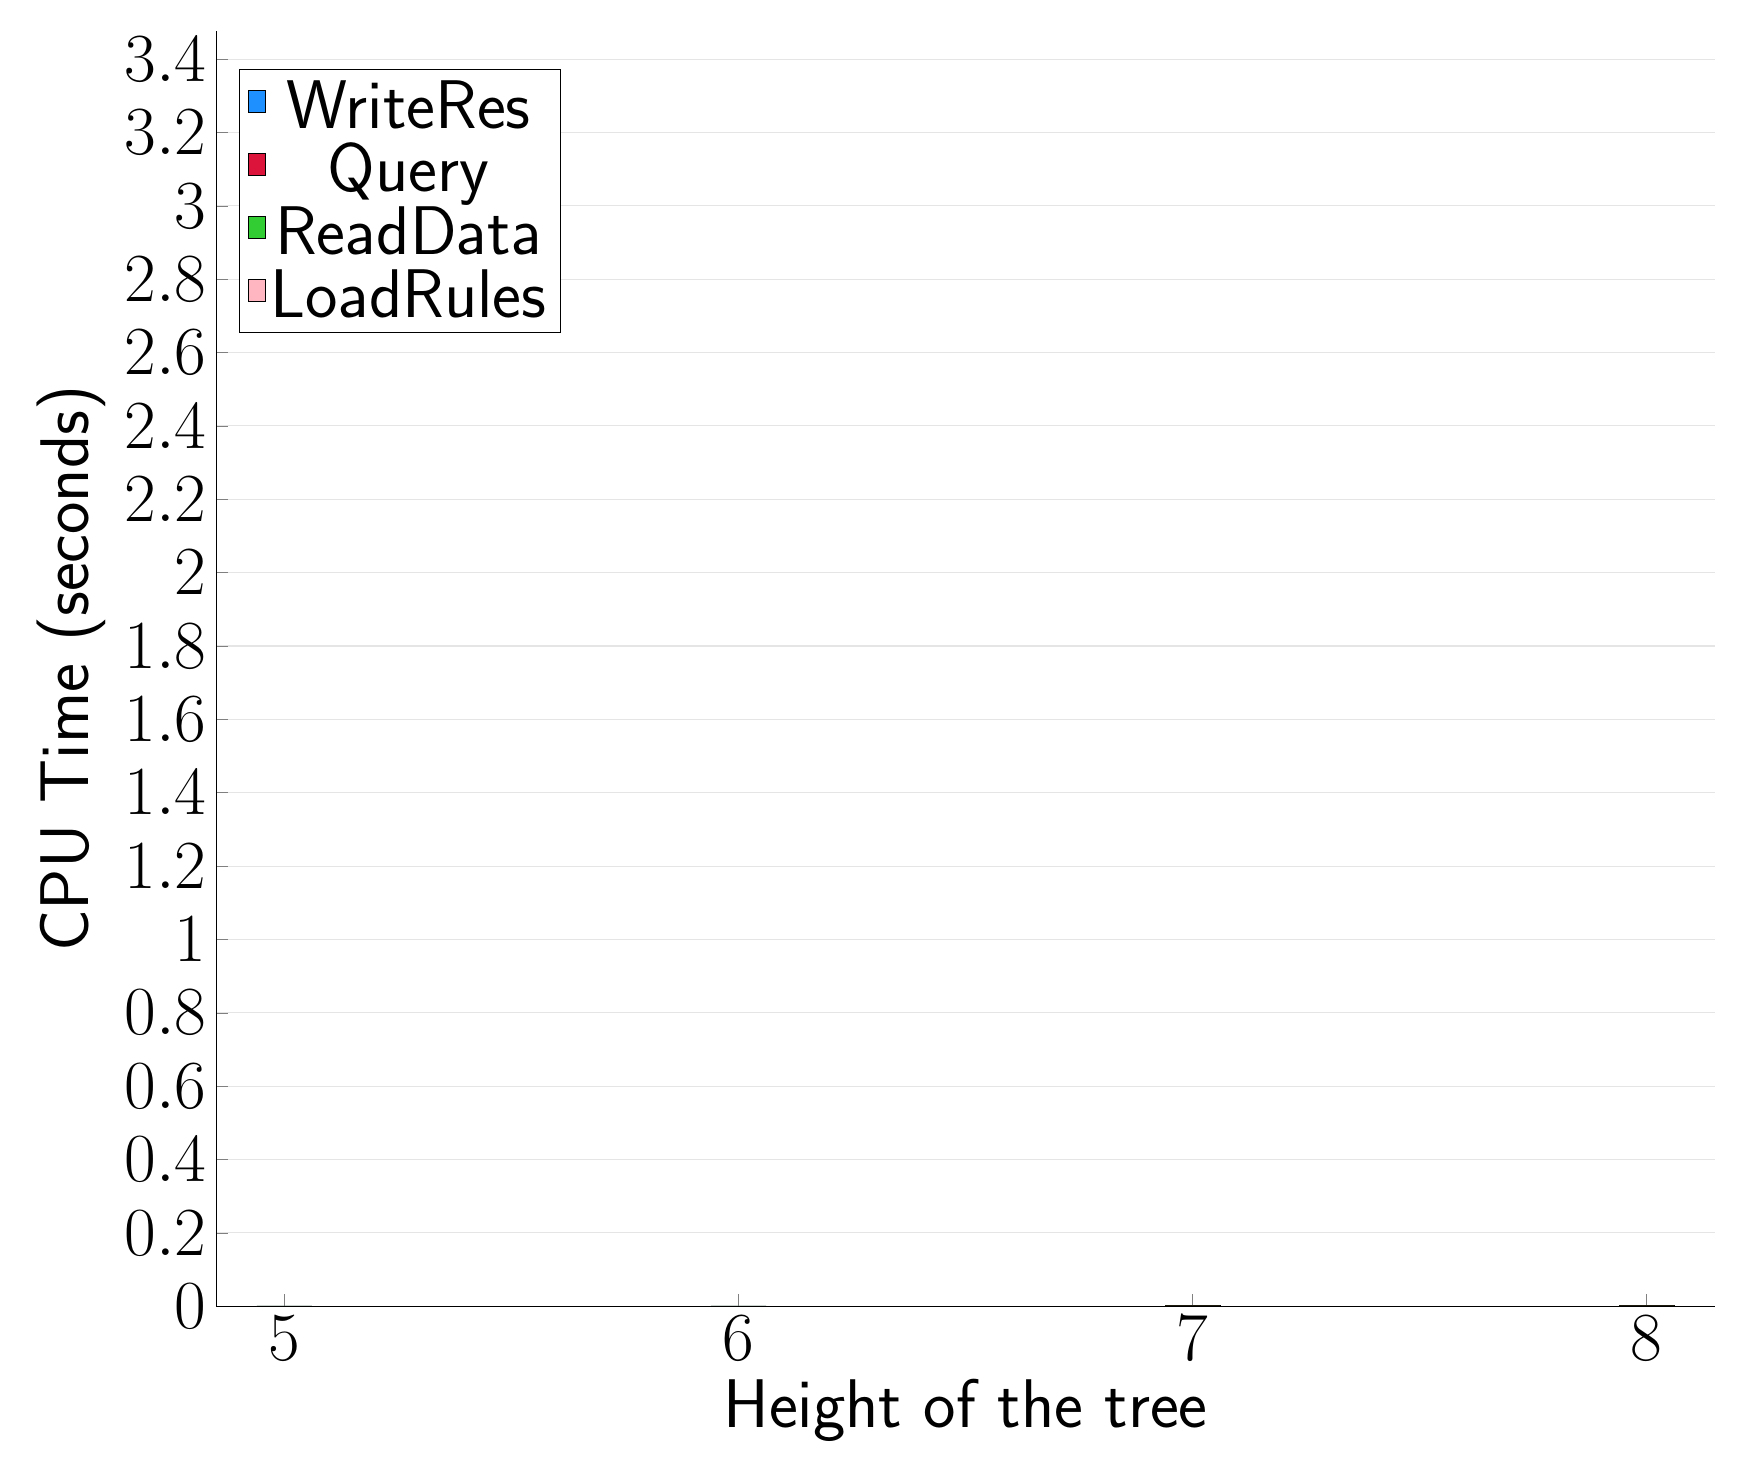
\begin{tikzpicture}
\begin{axis}[
   ybar stacked,
   width=1.7\textwidth,
   bar width=0.7cm,
   ymajorgrids, tick align=inside,
   major grid style={draw=gray!20},
   xtick=data,
   ymin=0, ymax=3.477,
   axis x line*=bottom,
   axis y line*=left,
   enlarge x limits=0.05,
   legend style={
       at={(0.23, 0.97)},
       anchor=north east,
       legend columns=1,
       font=\Huge,
   },
   ylabel={CPU Time (seconds)},
   xlabel={Height of the tree},
   label style={font=\Huge},
   tick label style={font=\Huge},
]
\addlegendimage{fill=DodgerBlue, draw=black, line width=0.2pt}
\addlegendentry{WriteRes}
\addlegendimage{fill=Crimson, draw=black, line width=0.2pt}
\addlegendentry{Query}
\addlegendimage{fill=LimeGreen, draw=black, line width=0.2pt}
\addlegendentry{ReadData}
\addlegendimage{fill=LightPink, draw=black, line width=0.2pt}
\addlegendentry{LoadRules}
\addplot +[fill=LightPink, draw=black, line width=0.2pt] coordinates {
(5, 0.000626)
(6, 0.0006193)
(7, 0.0005992000000000001)
(7, 0.0006191000000000002)
(7, 0.0006285999999999997)
(8, 0.0006097)
(8, 0.0006138999999999997)
(8, 0.0006213000000000003)
};
\addplot +[fill=LimeGreen, draw=black, line width=0.2pt] coordinates {
(5, 0.00015739999999999998)
(6, 0.00018460000000000029)
(7, 0.0002425000000000001)
(7, 0.00023899999999999993)
(7, 0.00024559999999999984)
(8, 0.00034490000000000004)
(8, 0.00035350000000000014)
(8, 0.00036599999999999946)
};
\addplot +[fill=Crimson, draw=black, line width=0.2pt] coordinates {
(5, 2.319999999999961e-05)
(6, 4.119999999999993e-05)
(7, 8.46999999999997e-05)
(7, 8.470000000000022e-05)
(7, 8.800000000000035e-05)
(8, 0.0001861000000000006)
(8, 0.00019009999999999974)
(8, 0.0001899000000000008)
};
\addplot +[fill=DodgerBlue, draw=black, line width=0.2pt] coordinates {
(5, 0.00015960000000000022)
(6, 0.0003096000000000005)
(7, 0.000655)
(7, 0.0006519999999999996)
(7, 0.0006555999999999995)
(8, 0.0014469999999999995)
(8, 0.0014550000000000003)
(8, 0.0014720999999999992)
};
\end{axis}
\end{tikzpicture}

\end{document}
